

% \begin{figure*}[th!]
%     \centering
%     \subfloat[Non-CPS-enhanced evacuation, with evacuees navigating to the closest exit, possibly past danger zones.]{
%       \centering
%       \includegraphics[width=0.49\textwidth]{img/fireEvac.jpg}
%       \label{fig:navigation_no_CPS}
%     }
%     \hfill
%     \subfloat[A birdseye view of a fire-evacuation using visual diffing. Ghosts represent a previous run, whilst solid grey people represent the live run. Coloured circles and lines represent node status and transmissions, respectively.]{
%         \centering
%         \includegraphics[width=0.49\textwidth]{img/CPSBirdseye.png}
%         \label{fig:birdseye_evac}
%     }
%     \caption{A normal evacuation vs a CPS-enhanced evacuation with visual diffing support.}
%     \label{fig:fire_evac_diff}
% \end{figure*}

% In the rest of this section we introduce DejaVu and explain in more detail the high-level visual diffing features which make DejaVu unique from the current state-of-the-art simulators, before describing the design and implementation of these features.

% \section{DejaVu - A Visual Diffing, 3D Virtual World CPS Simulator}
% % DejaVu was designed and built to solve the need for improved tools and methods for developing, testing and analysing cyber-physical systems in their target environments. Traditional simulation in isolation of the environment limits exposure to real-world issues, forcing developers to ``fudge'' interactions between the CPS and world, creating stubs for sensors or feeding in real or hand-crafted sensor data. These stop-gap measures are not only time-consuming thus limiting possible test coverage, but also increase the transfer gap between simulation and the real-world, where code needs significant change to move from simulation to deployment and back.

% % DejaVu bridges the gap between simulation and deployments, providing a virtual world to virtually deploy real code and simulate the interactions between a CPS and the environment. Using the Unreal engine 4, DejaVu can enable developers to create living 3D virtual worlds, grounded by realistic physics, lighting, sound, people and crowds.
% DejaVu is a 3D co-simulator platform for CPS and WSN, designed for running and comparing multiple simulation runs of a system in parallel. DejuVu is built using Cooja, a multi-level WSN simulator for Contiki-based nodes, and Unreal Engine 4 (UE4), a 3D game engine, providing a virtual world to virtually deploy real code and simulate the interactions between a CPS, the environment and virtual crowds. DejaVu can be used in both indoor and outdoor settings.

% DejaVu can efficiently record days of simulation data, including data from the virtual environment, sensors and radio network, enabling a full reconstruction of test scenarios for later playback, review and analysis. Unlike video recordings, using this reconstruction, developers are able to move through not only time but also space within recorded simulations, stopping, rewinding and fast-forwarding to review recorded simulations from any point of view at any point in time. To aid with traversing and analysing recordings, developers can select predefined events which DejaVu can watch for; when detected, a checkpoint is logged, enabling reviewers to at a glance see when events of interest have occurred and instantly replay them. DejaVu can also compare recordings in real-time, overlaying and highlighting differences between the current simulation and previously recorded runs, such as battery usage, radio utilisation/interference, movement, as well as other sensor readings.


% DejaVu simulations contain a number of nodes, which each have a corresponding representation in both Cooja and UE4, virtual and physical, respectively. For each node: Cooja simulates the software and radio components; UE4 simulates the physics for a nodes physical location and movement within the environment, provides visual representations of sensor devices and simulates the sensor interactions with the environment and people e.g., motion detection, fire detection.

% Whilst DejaVu is currently configured for use with Contiki's Cooja WSN simulator and UE4, DejaVu's architecture is agnostic and independent from these tools; in fact, it is designed to coordinate and compose multiple different simulators and tools.

% %
% % \subsection{Phenomena-on-demand}
% % In order to better test and understand sensor network applications in the real-world, developers often need to wait for or even force desired phenomena to occur and then observe how their system reacts. However, exercising control over the real-world can be a difficult and time- consuming challenge, and sometimes not possible (e.g., fire), due to health and safety concerns.
% % Using DejaVu, developers can take direct control of a virtual person or script realistic virtual crowds to carry out tasks, such as walking between points, avoidance, following or interacting with objects. Figure \ref{fig:birdseye} shows people walking up and down a corridor, avoiding each other’s path. Unlike using trace data, genuine or created, developers can easily tweak scenarios, such as moving devices, people or adjusting behaviour, to test subtle or significant variations in the rest of the system.



% \subsection{Time Control}
% When testing a CPS, time is a key factor: how long will \textit{mote 1} last for, what happened at time \textit{t}, how long did task \textit{x} take to complete, etc. Traditional methods for carrying out tests in the real world or simulations only allow observers to observe an event once live, or record an event from one or more fixed perspectives and then view only exactly what was in view when recording. This has obvious limits when it comes to live and post-test analysis. If events or data are missed, not recorded or out of view, then tests may need to be re-run, data approximated or interpolated. DejaVu supports multiple time control features, including pausing and fast-forwarding live simulations, as well as recording simulations for later playback and review.

% During a live simulation time can be paused, giving developers more time to fully observe the current state of the simulation, including moving around the 3D environment, before resuming. Time can also be fast-forwarded, reducing the real-world time for a simulation to be carried out. These two time control features enable developers to become more efficient and effective in carrying out live simulations.

% To aid in post-simulation review and analysis, everything within a simulation run can be recorded, saved and played back later, including data on people, objects, sensors, network traffic, etc. Unlike a video recording of a simulation visualisation, which provides only one fixed viewpoint into a simulation, DejaVu, using the recorded data, can completely reconstruct the simulation, enabling developers to review the simulation from any viewpoint at any point in time. This gives developers the power to investigate the simulation for events missed the first time or to simply change perspective to better understand a phenomena from another angle. Similarly, analytical filters and effects can also be retroactively applied, providing new views into recorded simulations.

% Similarly in DejaVu, instead of viewing simulations in isolation (\ref{fig:navigation_no_CPS}), developers can visual diff two simulations using ghosts, as shown in figure \ref{fig:birdseye_evac}, to show how differently crowds of people move.

% \subsection{Visual Diffing Techniques: Ghosts and Colour}
% Often when testing cyber-physical systems, either deployed in the wild or in simulation, developers are attempting to spot particular events, patterns or phenomena and compare these to previous observations or a baseline.

% For real world deployments, we are limited to what we can see through visual interfaces, external physical outputs or textual data logs. Similarly, by simply looking at the cyber-physical system in situ it is very difficult to observe activity and interaction between nodes. On top of this, trying to compare different test runs visually is extremely hard, without resorting to data logging and graphing.

% Like in the real world, within the simulated virtual world observing a system as-is can be just as difficult. However, because it is virtual, we can also enhance our view of it, super-imposing or overlaying information that would otherwise hidden from view, such as radio traffic, node stats, or sensor readings.

% Taking this one step further, using a recording saved earlier, the simulator can simultaneously run one or more simulations in parallel, enabling observers to visually compare or ``diff'' them directly. However, the difficulty arises in how to represent the non-visual data in intuitive ways. Depending on the type of data being compared, DejaVu presents diffs in multiple ways, appropriate to the data type.

% In a 3D world the simplest data to compare visually is position. When comparing two runs, a live and recorded run, movable physical elements from both can be shown simultaneously. To aid in differentiating elements of each simulation, the recorded run's elements are shown as ghosts, translucent in appearance which don't interact or collide with objects in the live simulation and simply repeat state-by-state what was recorded. This provides immediate visual clues to where simulation runs differ, useful in cases where the mobility of people or objects within it are of interest, such as in a observing crowd movement in an evacuation scenario or navigation decisions for domestic cleaning robots.

% To further improve this, additional visual effects can be used to filter out the visual noise. For example, when objects and their ghost stay within a set distance of one another, their colour is desaturated, however, when they breach this limit, they are visibly highlighted in colour, making it clear which objects are of interest.

% For meta-data, which is not typically visible on the surface of a node, such as node stats or sensor readings, we need to be more creative and take advantage of the customisation aspects of the 3D virtual world. We have created several techniques to visually signal differences between a live and recorded run: to simply alert the observer we can cause the whole device to periodically illuminate a particular colour, and simultaneously desaturate the others to further enhance the observability of it e.g., a node flashes red to signify its status is different between the two runs at the current time slice; alternatively, the simulator can also illuminate the device using a gradient of colours, signifying the intensity of the difference being observed between the two runs for a particular device e.g., nodes illuminate on a range from yellow to red based on the power difference between two runs, highlighting which nodes are affected the most. Other techniques include changing the size of devices based on the size of change, or shaking nodes.


% \subsection{Checkpoints: needles in a haystack}
% Utilising faster-than-real-time simulation, developers can run and record simulations up to three times faster than real-time. Thus, developers can run and review a virtual day within 8 hours of real time. However, this poses a problem for reviewing and analysing these long simulated runs, which can be akin to looking for a needle in a haystack when trying to find issues, key events or behaviours to analyse whether or not a system is operating correctly.

% To resolve this problem, in DejaVu developers can add an event observer to the simulation, which detects when a particular condition within the simulation is met. For example, a developer may be interested when a node's power level drops below a threshold, or when a sensor is activated. Upon triggering an event observer, the current snapshot is tagged as a checkpoint with the event type. When the simulation is replayed, the developer can then skip directly to any of the event checkpoints that were generated, highlighting snapshots of interest. Of course, developers can then choose to investigate both in time and space around this checkpoint, rewinding or fast-forwarding, as well as moving around the virtual world.

% \section{Design}

% \subsection{Co-simulator}
% DejaVu uses a publish-subscribe event system: in which a plugin for each component publishes or subscribes to events of interest. For example, the Unreal engine publishes sensor positions in the 3D virtual world, to which Cooja subscribes, thus updating it's radio interference model with every new position update. This approach enables the platform to be flexible and modular, allowing multiple components to publish and subscribe to information simultaneously, and for new features, tools or extensions to be added easily.

% % \begin{figure}[ht]
% %   \centering
% %   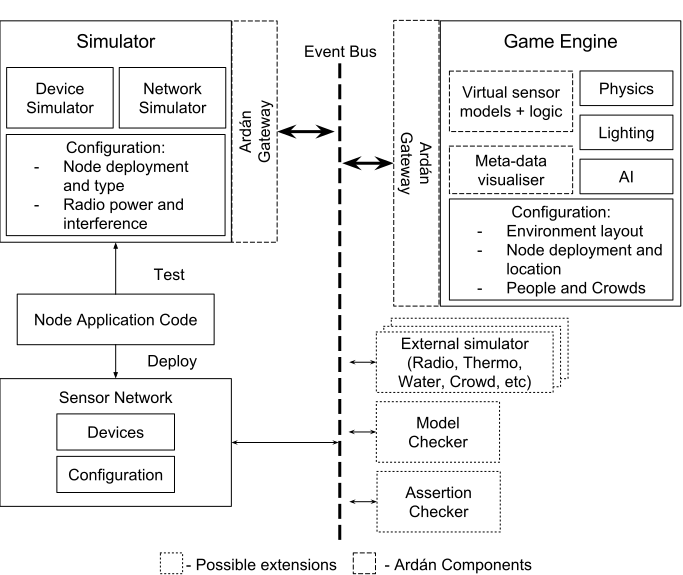
\includegraphics[width=0.5\textwidth]{img/architecture.pdf}
% %   \caption{Ard\'{a}n architecture}
% %   \label{fig:architecture}
% % \end{figure}
% %
% % While the goal of this work is to build an improved simulation experience for testing sensor network applications, we also want to create an architecture that can support future integration of tools to further improve the field of sensor network application testing.
% %
% % Thus, rather than integrate the systems directly, our approach uses a network event bus and common schema to describe information passed between the different sub-systems. This approach reduces the tight coupling between components, allowing individual components to be swapped out or new ones added. We envision the use of tools such as model checking, statistical analysis, unit-testing and advanced simulation for radio and environmental properties.
% %
% % The WSN simulator (Cooja), performs all application and network simulation for the co-simulation and is configured with a set of nodes with their 3D location and application code to run. As the application code is run in real-time, any sensor- or actuator-based hardware requests, such as sensor reads and actuator commands, are published to the event-bus, which the 3D game engine receives and performs in the virtual environment.

% % Within the Unreal Engine we have modelled a 3D office environment and created a several components to support deploying virtual sensor networks, including device and sensor 3D models, hardware abstractions for the virtual sensors and actuators to sense the virtual world and report back to the simulator over the network bus. Similarly within the Cooja simulator we have modified the simulated hardware to communicate to our virtual hardware in the Unreal Engine via the event-bus.

% \subsection{Recording}
% \label{ssub:time_control}
% In order to perform time-control functions, DejaVu records both observable and unobservable behaviour within a simulation, including physical information about an object's position, trajectory and rotation, as well as metadata and state associated with any devices, sensors and the radio environment e.g., power usage, sensor readings and radio transmissions. Recording both observable and unobservable information ensures replays can be fully reconstructed or later modified to include new views or filters over the information and world.

% To optimise the amount of memory used, DejaVu's snapshots only contain data about objects whose state has changed since the last snapshot, thus ensuring memory is not wasted recording duplicate data. However, even when using this method of recording, memory size still becomes an issue when recording a large number of objects over an extended period of time, e.g., 60 people + 20-30 sensors over a 24hr period consumes 36GB, exceeding the RAM available on even high-end machines.

% Thus, to further reduce the memory used, DejaVu utilises a segmented compression scheme, seen in figure \ref{fig:compression}. The continuous stream of snapshots are divided into segments of a fixed size. Segments which are not currently being played are compressed and written to storage. Segments are lazily loaded back into memory and decompressed when necessary. Using this scheme DejaVu saves a considerable amount when storing these recordings, up to 30x improvement as shown in figure \ref{tab:offline-storage}. Using this technique, DejaVu can record arbitrarily long simulations.

% \begin{figure}[ht]
%   \includegraphics[width=0.5\textwidth]{img/DejaVuCompression.pdf}
%   \caption{Segmented compression scheme employed by DejaVu to reduce in-memory usage.}
%   \label{fig:compression}
% \end{figure}

% To prevent this scheme from negatively impacting the performance when skipping back and forth through a recording, segments before and after the current segment are preemptively loaded. The pre-loading distance can be adjusted to balance the performance and storage needs. For long-distance scrubbing, i.e., skipping hours or days, each segment is time-stamped with the start- and end-times of the snapshots held within, providing improved performance when indexing into the correct segment.

% Using this memory efficient scheme, DejaVu is able to record week-long simulations which would far surpass the available memory on even a high-end workstation. Because of the segmented compression scheme, DejaVu can load multiple recording streams simultaneously, opening up the possibility to replay, diff and compare multiple runs in real-time.

% \begin{table}[h]
% \centering
% \begin{tabular}{|l|l|l|l|l|}
% \hline
%            & 1min  & 1hr    & 24hr  \\ \hline
% raw        & 40MB  & 1.5GB  & 36GB  \\ \hline
% compressed & 1.6MB & 45.1MB & 1.1GB \\ \hline
% \end{tabular}
% \caption{Size comparison between raw and compressed snapshots saved to disk, varying in length.}
% \label{tab:offline-storage}
% \end{table}
% % 7 252GB 8GB
% % 10mins 30mins   47mins
% % r 272.4MB 834MB 1.25GB
% % c 8MB 24.5MB    36.5MB


% \subsection{Visual Diffing}
% DejaVu supports visual diffing a recorded simulation against another recording or a live simulation. Visual diffing utilises the simulation recording and replaying methods described in the previous section, allowing more than one simulation stream to be played back in memory simultaneously.
% \begin{figure*}[t!]
%     \centering
%     \subfloat[CPS-enhanced evacuation diffed with non-enhanced ghosts. Evacuees are being directed to exits via safe routes.]{
%       \centering
%       \includegraphics[width=0.49\textwidth]{img/fireEvacCPS2.png}
%       \label{fig:cps_diff}
%     }
%     \hfill
%     \subfloat[A person evacuating chooses two different paths in different runs based on CPS assistance, the ghost shows the same person taking a different route in a previous run.]{
%         \centering
%         \includegraphics[width=0.49\textwidth]{img/fireevacghost.png}
%         \label{fig:path_navigation_diff}
%     }
%     \caption{Different visual diffing techniques for differentiating different aspects of simulation runs.}
%     \label{fig:diff_features}
% \end{figure*}

% When replaying and diffing two simulations, each recordable object (device, person or moveable object) in DejaVu keeps track, within its log of snapshots, of a pointer to the snapshot closest to the current replay time, updated at each tick in the game engine. DejaVu runs the selected diff on each relevant corresponding object in both simulation streams, which compares the current snapshot of each object to determine the differences. Developers can also define the difference threshold, specifying the closeness of the objects' values before they are considered different. Currently, DejaVu supports a library of built in diffing functions, including location, device sensor state (motion-, fire-detection), LED state and radio usage.

% The results from each diff function are then linked to different visual diffing features, e.g., location difference is shown through ghosting (figure \ref{fig:cps_diff}) and/or visual tracks (figure \ref{fig:path_navigation_diff}), discrete differences through a colour change of the object and continuous differences by a colour gradient. Multiple visual features can also be applied to a single diff function, such as using ghosting for showing location differences, but also colouring the corresponding objects should they differ by a developer-defined threshold, visually alerting the developer to points of interest. New visual features can be added and swapped in to experiment with visual techniques for representing differences. Similarly, we also envision the use of sound alerts or
% % When diffing two simulations, objects within the world are divided into three types: stationary objects, which remain at a fixed position and do not contain state; movable objects, which can be moved but contain no state; and devices, which can be stationary or movable and contain state. Between simulations stationary objects do not change, thus, only one instance is necessary in the environment. A movable object's position could be different between simulations, thus, duplicating the object is necessary in order to show where the object is comparatively between simulations.

% \section{Case study: Fire Evacuation}
% \label{sec:case_study}
% To demonstrate DejaVu's features we developed a case study which focuses on the use of a cyber-physical enhanced fire detection and evacuation system for large buildings with multiple corridors and exit routes, such as offices or shopping malls. Previous work by \cite{doi:10.1093/comjnl/bxq012,7152824} has demonstrated the use and benefit of utilising a 2D evacuation simulator to develop new cyber-physical systems to enhance detection and evacuation, ensuring people are directed away from high-risk areas, reducing congestion at critical paths and providing detailed information for emergency crew to locate areas of high-interest. Our case study utilises the algorithm from this approach, to demonstrate and evaluate the unique simulation features of DejaVu, including 3D analysis, playback, diffing and checkpointing.

% \begin{figure}[bht]
% \begin{lstlisting}[style=CPSCAL]
% broadcast msg {ID, dist}
% select:
%   waiton msg {ID, dist}:
%     routes[ID] = dist + 1
%     effectiveDist = min(dist+1, effectiveDist)
%     if changed:
%       broadcast msg {ID, effectiveDist}
%   waiton msg {ID, FIRE}:
%     routes[ID] = FIRE
%     effectiveDist = min_hazard(routes)
%     broadcast msg {ID, effectiveDist}
%   waiton sensor {FIRE}:
%     broadcast msg {ID, FIRE}
% \end{lstlisting}
% \caption{Pseudo-code for distributed evacuation CPS}
% \label{code:algo}
% \end{figure}

% The algorithm, shown in pseudo-code form in figure \ref{code:algo}, runs on each node within the network. Each node first broadcasts its distance to an exit; upon receiving a distance message, a node recalculates its shortest path to an exit; upon receiving a fire message, a node removes the senders path and recalculates the shortest distance to an exit taking into consideration the distance to the closest exit via a path and that path's hazard risk based on its distance to the nearest hazard; lastly, if a node receives a fire message from its own sensor, it broadcasts the fire alert to the rest of the network. Each node knows the direction of its nearest neighbours at deployment time, thus, using light indicators, observers can be directed along the calculated safe routes.

% Using DejaVu, we interactively programmed the evacuation system, testing and debugging our initial distributed navigation algorithm using virtual agents to react to virtual emergency fire evacuations.
% Using the replay and diff features, we were able to observe the differences that occur between different runs of the evacuation. For our analysis we focused on observing evacuation navigation between simulation runs, i.e., agent movement in reaction to the algorithm direction. Further examples of DejaVu's diffing capabilities are show in the appendix.

% Upon adapting the fire evacuation algorithm, we are able to use DejaVu to visually observe how it affects evacuation navigation. Before using the algorithm, evacuees would simply navigate to the exit closest to them, signposted by static exit signs, as shown in figure \ref{fig:navigation_no_CPS}, unless they encounter a fire. When the CPS is deployed, shown in figure \ref{fig:cps_diff}, evacuees are guided to the nearest safe exit, which may be longer than the shortest route, because of a fire hazard en route. Using DejaVu, the difference between these two scenarios is clear, in which the unaided scenario can be seen played out by the ghosts, whilst the current CPS-enhanced scenario avoids directing people towards the fire, using dynamic floor signs - pointing the people towards the safe route.

% Sensors can also be seen as white cuboids mounted along the corridor walls in figure \ref{fig:cps_diff}, detecting fire and relaying information between themselves according to the algorithm. The double coloured circles and lines signify radio traffic from one node to another, whilst the smaller coloured rings and LEDs reflect the status LEDS the node; these visual overlays expose more information typically hidden from sight in the real-world.


% \section{Performance}
% \label{sec:evaluation}
% Along with providing visual and diffing benefits, DejaVu also needs to be able to run and record at real-time or faster, with a realistic number of devices, people and activity within the environment, in order for development time to be significantly reduced when compared to traditional methods, such as testbeds or simulations.

% For device simulation, Cooja was loaded with Cooja native motes, which are Contiki OS-based applications compiled to run natively on the host machine. These offer a significant speed boost of several orders of magnitude when compared to emulated motes at the cost of hardware accurate simulation.

% Within the game engine, maintaining a high frames-per-second (FPS), above 30FPS, ensures a smooth and consistent physics simulation within the virtual world. On top of this when recording the simulation at faster than real-time, the FPS in the simulated world is reduced proportionally, to 1/x, where x is the speed up in the real-world. To ensure smooth playback and physics in the replay, a high FPS is needed e.g., 60FPS for x2 speed.

% Performance tests were carried out with both UE4 and Cooja co-located on the same machine of the following spec: Xeon E5 1650 6Core with HT, 16GB RAM, 256GB SSD and a sufficiently powerful (MSI GeForce GTX 970) graphics card to support the game engine.

% The performance test utilised the evacuation scenario described previously, with 30 sensors deployed and 60 evacuees. When run the simulation maintained an average of 75FPS with Cooja maintaining a constant x1.0 real-time factor; which demonstrates DejaVu can support realistically sized simulation with the use of large numbers of agents and devices simultaneously, whilst maintaining a consistently high FPS, ensuring fluid and efficient simulations.

% To further improve simulation performance (FPS), simulations can be recorded at lower visual fidelity, e.g., choosing a lower resolution and texture sizes. When played back, the visual quality can be increased, improving the observation view without impacting the results of the simulation.





% \section{Conclusion and Future Work}
% In this paper we presented DejaVu, a 3D co-simulator supporting full 3D reconstruction and visual diffing of live and recorded CPS deployment simulations. We demonstrated the significance and capabilities that the visual diffing features provide through the use of an evacuation case study. DejaVu enables developers to quickly analyse simulated runs, highlighting points of interest and differences between runs with full time-control, seamlessly within the simulation itself.

% In future we envision extending the support for filtering and diffing, utilising event-stream processing to detect events and complex patterns of events. With the recent developments in virtual reality (VR) and mixed-reality (MR) technologies, VR and MR will provide new and exciting ways to support virtual testing and deployment, both in terms of the human-in-the-loop scenarios for virtual experiment participants, as well as for developers experimenting with deployment layout and live analytics superimposed onto objects within the real environment.
